\documentclass[12pt]{article}

\fontfamily{lmss}
\usepackage{fullpage}
\usepackage{amsmath}
\usepackage{amsthm}
\usepackage{url}
\usepackage{multicol}
\usepackage{enumerate}
\usepackage{graphicx}
\usepackage{color}
\usepackage[labelfont=sc]{caption}
\usepackage{subcaption}
\usepackage[title]{appendix}
\usepackage{xcolor}
\usepackage{enumitem}
\usepackage{siunitx}
\usepackage{algorithm}
\usepackage{algpseudocode}
\usepackage{amssymb}

\usepackage{tikz}
\usetikzlibrary{graphs}
\usetikzlibrary{arrows.meta,shapes,shapes.geometric}
\usetikzlibrary{positioning, quotes}

\tikzset{
  % Two node styles for game trees: solid and hollow
  solid node/.style={circle,draw,inner sep=1.2,fill=black},
  hollow node/.style={circle,draw,inner sep=1.2},
  % styles for long branch labels
  left label/.style={above left,midway},
  right label/.style={above right,midway}
}

\usepackage{hyperref}
\hypersetup{
    colorlinks=true,
    linkcolor=blue,
    filecolor=magenta,      
    urlcolor=blue,
}

\usepackage{geometry}
\geometry{
  top=1in,            % <-- you want to adjust this
  bottom=1in,
  left=1in,
  right=1in,
  headheight=3ex,       % <-- and this
  headsep=4ex,          % <-- and this
}

\usepackage{lastpage}
\usepackage{fancyhdr}
\pagestyle{fancy}
\fancyhf{}
\renewcommand{\footrulewidth}{0.4pt}
\lhead{CS 486/686}
\rfoot{Page \thepage\ of \pageref{LastPage}}

\setlength{\parskip}{\baselineskip}%
\setlength{\parindent}{0pt}%

\usepackage{tcolorbox}
\tcbuselibrary{breakable}
\newenvironment{markscheme}
{
    \renewcommand{\parskip}{\baselineskip}
    \begin{tcolorbox}[
        colback=blue!10,
        colframe=blue!10,
        sharp corners,
        breakable
    ]
    \textbf{Marking Scheme:}
}
{
    \end{tcolorbox}
}

\newenvironment{sol}
{
    \renewcommand{\parskip}{\baselineskip}
    \begin{tcolorbox}[
        colback=magenta!10,
        colframe=magenta!10,
        sharp corners,
        breakable
    ]
    \textbf{Solutions:}
}
{
    \end{tcolorbox}
}

\newenvironment{example}
{
    \renewcommand{\parskip}{\baselineskip}
    \begin{tcolorbox}[
        colback=green!10,
        colframe=green!10,
        sharp corners,
        breakable
    ]
}
{
    \end{tcolorbox}
}

\lhead{CS 486/686}
\chead{Fall 2022}
\rhead{Assignment 2}
\cfoot{v1.0}
\lfoot{\copyright Blake VanBerlo 2022}

\title{CS 486/686 Assignment 2 \\ Fall 2022 \\ (86 marks) }
\author{Blake VanBerlo}
\date{Due Date: 11:59 PM ET on Tuesday, October 25, 2022}

\newcommand\independent{\perp\!\!\!\perp}

\begin{document}

\maketitle

% \section*{Changes}

% \begin{itemize}

% \end{itemize}

\newpage
\section*{Instructions}

\begin{itemize}
\item
Submit the signed academic integrity statement any written solutions in a file to the Q0 box in the A2 project on Crowdmark. \textbf{(5 marks)}.

\item Submit your written answers o questions 1 and 2 as PDF files to the Q1 and Q2 boxes respectively in the A2 project on Crowdmark. I strongly encourage you to complete your write-up in LaTeX, using this source file. If you do, in your submission, please replace the author with your name and student number. Please also remove the due date, the Instructions section, and the Learning goals section. Thanks!

\item Submit any code to \verb+Marmoset+ at \url{https://marmoset.student.cs.uwaterloo.ca/}. Be sure to submit your code to the project named \texttt{Final}. 

\item
No late assignment will be accepted. This assignment is to be done individually.

\item
Lead TAs: 
\begin{itemize}
\item 
Christopher Risi (\url{cjrisi@uwaterloo.ca})
\item
Dake Zhang (\url{dake.zhang@uwaterloo.ca})
\end{itemize}
The TAs' office hours will be scheduled and posted on LEARN and Piazza.
\end{itemize}



\section*{Learning goals}

{\bf Bayesian Networks}
\begin{itemize}
    \item Understand independence and conditional independence relationships in Bayesian networks.
\end{itemize}
{\bf Variable Elimination Algorithm}
\begin{itemize}
    \item Define factors. Manipulate factors using the operations restrict, sum out, multiply and normalize.
    \item Trace the execution of and implement the variable elimination algorithm for calculating a prior or a posterior probability given a Bayesian network.
\end{itemize}


\newpage

\section{Three Proofs (26 marks)}

\begin{enumerate}[font=\Large,label=(\alph*)]

    \item Recall that random variables $X$ and $Y$ are conditionally independent, given a third variable $Z$ if and only if:
    
    \begin{equation}
        P(X|Y \land Z) = P(X|Z)
        \label{eq:ci1}
    \end{equation}
    
    \begin{equation}
        P(Y|X \land Z) = P(Y|Z)
        \label{eq:ci2}
    \end{equation}
    
    \begin{equation}
        P(X \land Y|Z) = P(X|Z)P(Y|Z)
        \label{eq:ci3}
    \end{equation}
    
    Show that Equation~\ref{eq:ci3} follows from Equations~\ref{eq:ci1} and \ref{eq:ci2}. Justify each step of your proof.
    
    \underline{Hint:} you may find some of the probability rules from Lecture 6 to be useful.
    
    \begin{markscheme}
    (6 marks)
    
    \begin{itemize}
    \item
    (4 marks) Correct proof
    \item
    (2 marks) Each step is justified
    \end{itemize}
    \end{markscheme}
    
    \begin{sol}
        {\color{blue} 

            $P(X|Y \land Z) = P(X \land Y \land Z)/P(Y \land Z)= P(X|Z) $  - Conditional Probability from equation 2

            $P(X \land Y|Z) = P(X \land Y \land Z)/P(Z) $  - Conditional Probability  
            
            $ = P(X \land Y \land Z)/ P(Y \land Z) * P(Y \land Z)/P(Z) $  - Alegebra

            $ = P(X|Z) * P(Y \land Z)/P(Z) $  - Substitute Equation 2

            $ = P(X|Z)P(Y|Z) $  - Conditional Probability
        }   
        \end{sol}

    \item The \textit{Markov blanket} of random variable $X$ in a Bayesian network consists of the set of random variables that are parents, children, or parents of children of $X$. For a Bayesian network with random variables $\mathcal{S}$, let $B = \{B_1, B_2, ..., B_n\} \subset \mathcal{S}$ be the Markov blanket for $X \in \mathcal{S}$. See Figure~\ref{fig:markov_blanket} for an example.
    
    \begin{figure}[ht!]
        \centering
        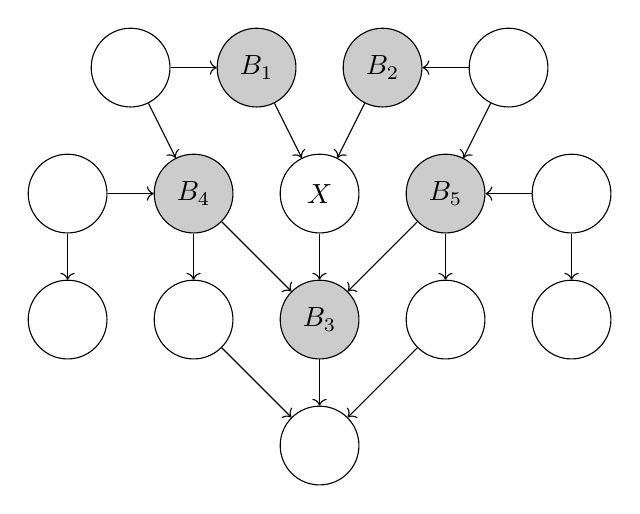
\begin{tikzpicture}[x=0.8cm,y=0.8cm]
            \tikzstyle{every node}=[draw,minimum size=1cm];
            \node[ellipse] (x) at (0, 0) {$X$};
            \node[ellipse,fill=black!20] (b1) at (-1, 2) {$B_1$};
            \node[ellipse,fill=black!20] (b2) at (1, 2) {$B_2$};
            \node[ellipse,fill=black!20] (b3) at (0, -2) {$B_3$};
            \node[ellipse,fill=black!20] (b4) at (-2, 0) {$B_4$};
            \node[ellipse,fill=black!20] (b5) at (2, 0) {$B_5$};
            \node[ellipse] (z1) at (2, -2) {};
            \node[ellipse] (z2) at (-2, -2) {};
            \node[ellipse] (z3) at (-3, 2) {};
            \node[ellipse] (z4) at (3, 2) {};
            \node[ellipse] (z5) at (-4, 0) {};
            \node[ellipse] (z6) at (4, 0) {};
            \node[ellipse] (z7) at (0, -4) {};
            \node[ellipse] (z8) at (-4, -2) {};
            \node[ellipse] (z9) at (4, -2) {};
            \path[draw] [->] (b1) -- (x);
            \path[draw] [->] (b2) -- (x);
            \path[draw] [->] (x) -- (b3);
            \path[draw] [->] (b4) -- (b3);
            \path[draw] [->] (b5) -- (b3);
            \path[draw] [->] (z3) -- (b1);
            \path[draw] [->] (z4) -- (b2);
            \path[draw] [->] (z5) -- (b4);
            \path[draw] [->] (z6) -- (b5);
            \path[draw] [->] (b4) -- (z2);
            \path[draw] [->] (b5) -- (z1);
            \path[draw] [->] (b3) -- (z7);
            \path[draw] [->] (z1) -- (z7);
            \path[draw] [->] (z2) -- (z7);
            \path[draw] [->] (z3) -- (b4);
            \path[draw] [->] (z4) -- (b5);
            \path[draw] [->] (z5) -- (z8);
            \path[draw] [->] (z6) -- (z9);
        \end{tikzpicture}
        \caption{An example of a Bayesian network with its Markov blanket shaded grey.}
        \label{fig:markov_blanket}
    \end{figure}
    
    Show that $X \independent Y \,|\, B$, $\forall \; Y \in \mathcal{S} \setminus B$. In other words, show that $X$ is conditionally independent of every other variable in the network, conditioned on its Markov blanket.
    
    \underline{Hint:} Consider using the fundamental conditional independence relationships discussed in Lecture 8.
    
    \newpage
    \begin{markscheme}
    (10 marks)
    \begin{itemize}
    \item
    (8 marks) Correct proof
    \item
    (2 marks) Proof is succinct and easy to understand
    \end{itemize}
    \end{markscheme}

    \begin{sol}
        {\color{blue} 
        For X to be conditionally independent with any node N given B , there should not be a path from X to N that does not go through B. Since B includes all children and parents of X, this holds for all N and thus X is conditionally independent of every variable in the network,conditioned on its Markov blanket
        }
    \end{sol}
    
    \item Not all the random variables in a Bayesian networks are always required to answer a probabilistic query. In fact, all variables that are not ancestors of query variables or evidence variables are irrelevant to the query. Let $Q = \{Q_1, \hdots, Q_m\}$ be the set of query variables and $e = \{e_1, \hdots,e_n\}$ be the set of evidence variables. Prove that the Variable Elimination Algorithm (VEA) returns the same distribution for some query $P(Q|E)$ if all irrelevant variables are pruned from the Bayesian network.
    
    \underline{Hint:} try a direct proof. Show that a particular ordering of hidden variable elimination results in the same final distribution returned by the normalization operation.
    
    \begin{markscheme}
    (10 marks)
    
    \begin{itemize}
    \item
    (8 marks) Correct proof
    \item
    (2 marks) Proof is succinct and easy to understand
    \end{itemize}
    \end{markscheme}

    \begin{sol}
        {\color{blue} 
            TODO
        }
        \end{sol}

\end{enumerate}


\section{The Variable Elimination Algorithm (55 marks)}

You will implement the variable elimination algorithm to perform inference in Bayesian networks with discrete random variables.

We have provided four Python files. Please read the detailed comments in the provided files carefully.

\begin{table}[ht!]
    \centering
    \begin{tabular}{llp{12cm}}
         $1.$ & \verb+factor.py+ & Defines a factor class for VEA. {\bf Do not change this file.} \\[5pt]
         $2.$ & \verb+vea.py+ & Contains empty functions for VEA operations. You will implement all of the functions in this file. {\bf Do not change the function signatures.} \\[5pt]
         $3.$ & \verb+example.py+ & Provides a demonstration of how to define the factors for a Bayesian network (for the Holmes scenario) and execute the variable elimination algorithm. \\
    \end{tabular}
    \label{tab:files_desc}
\end{table}


Here are some tips for implementing the variable elimination algorithm:

\begin{enumerate}
    \item \verb+restrict()+: Consider using splicing operations or \verb+take+.
    \item \verb+multiply()+: Consider using the \verb+numpy+ broadcasting rules to multiply multidimensional arrays of different shapes.
    \item \verb+sum_out()+: Consider using the \verb+sum+ operation.
    \item You may find it helpful to print the VEA operations and intermediate factors. See Appendix~\ref{apx:vea_output_format} for tips on printing the output of VEA. Note that this is optional.
\end{enumerate}

% QUESTIONS %%%%%%%%%%%%%%%%%%%%%%%%%%%%%%%%%%%%%%%%%%%%%%%%%%%%%%%%%%%%%%%%%%%%%%%%%%%%%%%%%%%%%%%%%%%%%%%%%%%%%%

{\bf Please complete the following tasks.}

\begin{enumerate}[font=\Large,label=(\alph*)]

\item 
Implement the empty functions in \verb+vea.py+. Zip and submit this file only on Marmoset.
    
\begin{markscheme}
(49 marks)

Unit tests:
\begin{itemize}
    
    \item \verb+normalize+ \\
    (1 public test + 2 secret tests) $\times$ 1 mark = 3 marks

    \item \verb+restrict+ \\
    (1 public test + 2 secret tests) $\times$ 2 marks = 6 marks
    
    \item \verb+sum_out+ \\
    (1 public test + 2 secret tests) $\times$ 2 marks = 6 marks

    \item \verb+multiply+ \\
    (1 public test + 7 secret tests) $\times$ 2 marks = 16 marks
    
    \item \verb+vea+ \\
    (1 public test + 5 secret tests) $\times$ 3 marks = 18 marks

\end{itemize}
    
\end{markscheme}

\begin{sol}
    {\color{blue} 
    Code submiited.
    }
\end{sol}

\item
Below is a Bayesian network that appears in a recent review of uncertainties in Bayesian networks with discrete variables (\href{https://www.sciencedirect.com/science/article/abs/pii/S0952197619303045}{Rohmer, (2020)}). The network is a probabilistic model of brain cancer diagnosis. Note that the example is meant to be illustrative, as the network is simple and the conditional probability tables are fictional. The random variables are defined below: \\

\begin{table}[ht!]
    \centering
    \begin{tabular}{l|l}
         Random Variable & Definition \\
         \hline
         MC & Metastatic cancer \\ 
         B & Brain tumour \\ 
         CT & CT scan is positive for brain tumour \\ 
         SH & Severe headache \\ 
         ISC & Increased serum calcium \\ 
         C & Patient falls into coma \\
    \end{tabular}
    \label{tab:random_vars}
\end{table}


\begin{center}
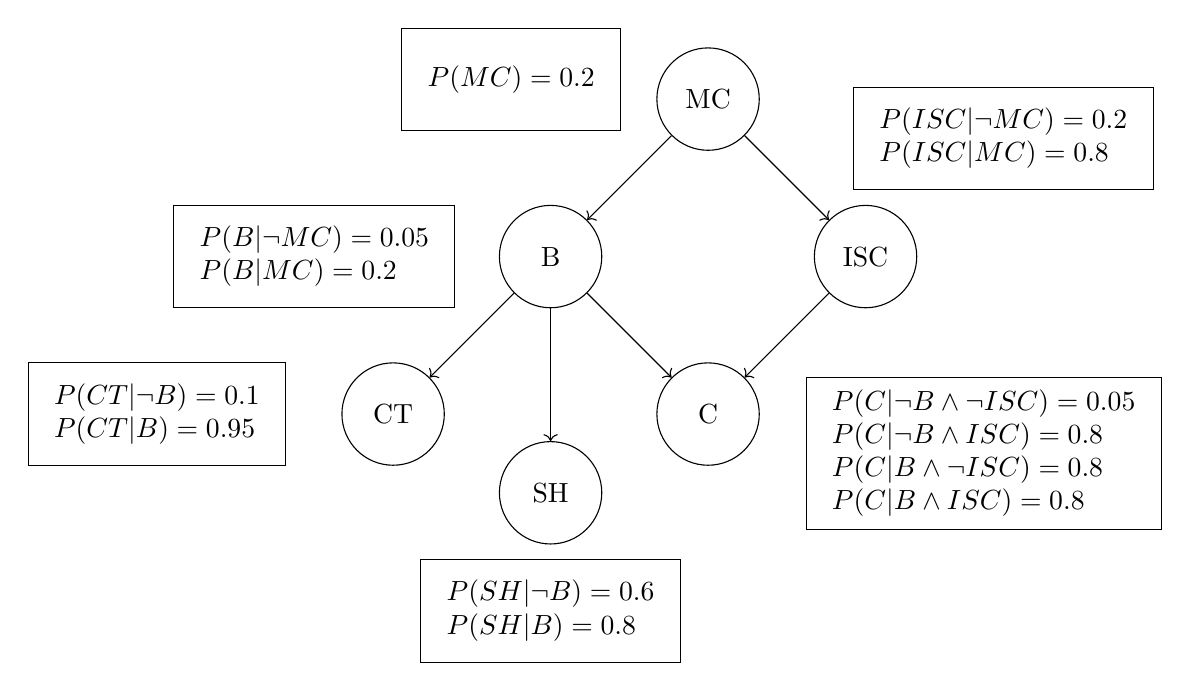
\begin{tikzpicture}
\tikzstyle{every node}=[draw,minimum size=1.3cm];


\node (tab-mc) at (-2.5,6.25) {
\begin{tabular}{l}
$P(MC) =0.2$ \\
\end{tabular}
};

\node (tab1) at (-5,4) {
\begin{tabular}{l}
$P(B | \lnot MC) =0.05$ \\
$P(B | MC) = 0.2$
\end{tabular}
};

\node (tab1) at (3.75,5.5) {
\begin{tabular}{l}
$P(ISC | \lnot MC) = 0.2$ \\
$P(ISC | MC) = 0.8$
\end{tabular}
};

\node (tab1) at (-7,2) {
\begin{tabular}{l}
$P(CT | \lnot B) = 0.1$ \\
$P(CT | B) = 0.95$
\end{tabular}
};

\node (tab1) at (3.5,1.5) {
\begin{tabular}{l}
$P(C | \lnot B \land \lnot ISC) = 0.05$ \\
$P(C | \lnot B \land ISC) = 0.8$ \\
$P(C | B \land \lnot ISC) = 0.8$ \\
$P(C | B \land ISC) = 0.8$ \\
\end{tabular}
};

\node (tab1) at (-2,-0.5) {
\begin{tabular}{l}
$P(SH | \lnot B) = 0.6$ \\
$P(SH | B) = 0.8$
\end{tabular}
};

\node[ellipse] (mc) at (0, 6) {MC};
\node[ellipse] (b) at (-2, 4) {B};
\node[ellipse] (isc) at (2, 4) {ISC};
\node[ellipse] (c) at (0, 2) {C};
\node[ellipse] (ct) at (-4, 2) {CT};
\node[ellipse] (sh) at (-2, 1) {SH};
\path[draw] [->] (mc) -- (b);
\path[draw] [->] (mc) -- (isc);
\path[draw] [->] (b) -- (ct);
\path[draw] [->] (b) -- (sh);
\path[draw] [->] (b) -- (c);
\path[draw] [->] (isc) -- (c);
\end{tikzpicture}
\end{center}

Using your implementation from the previous question, execute the Variable Elimination Algorithm to determine the probability that a patient has a brain tumour, given that their blood work shows an increased calcium concentration, and they do not report having severe headaches. Eliminate hidden variables in reverse alphabetical order. For example, you would eliminate $MC$ before $ISC$ and $CT$ before $C$. For each random variable's domain,  consider \verb+False+ as $0$ and \verb+True+ as $1$.

\begin{markscheme}
(2 marks)

\begin{itemize}
\item (2 marks) Correct answer
\end{itemize}
\end{markscheme}

\begin{sol}
    {\color{blue} 
    $P(B|ISC \land \lnot SH) = 0.0667$

    }
\end{sol}

\item
The complexity of VEA depends on the \textit{treewidth} of the Bayesian network, which is the maximum number of random variables in a factor after summing out a variable. The order in which hidden variables are eliminated impacts the treewidth, thereby impacting the complexity.

Use your implementation of VEA to evaluate the probability of metastatic cancer given that a patient's CT scan is positive for a brain tumour (i.e., $P(MC=1|CT=1)$). Do not prune the network. Execute VEA for each possible order of eliminating the random variables and note the treewidth in each case. Produce a histogram of the treewidths for each execution of VEA.

\underline{Hint:} You might find \verb+itertools.permutation()+ useful in determining the possible permutations of a list of strings.

\newpage
\begin{markscheme}
(4 marks)

\begin{itemize}
\item (3 marks) Plot is correct
\item (1 mark) Plot is clear
\end{itemize}
\end{markscheme}


\end{enumerate}

\begin{appendices}

\section{Printing the output of VEA}
\label{apx:vea_output_format}

You might find it helpful to print the output of the intermediate factors created during the execution of VEA. In our solution code, we print out each factor along with the steps of the algorithm when the \verb+verbose+ argument in \verb+vea()+ is set to \verb+True+. Below we provide guidance on how you could print the algorithm's intermediate steps to understand it and debug. Note that if you are asked to manually perform VEA on an exam, you will be asked to list your steps in a similar format.

Note that we are not marking your code for its console output --- only for the values returned by each function.

Print out a factor as \verb+f(A B E)+. Use \verb+f+ to denote the name of every factor. Print out the variables in {\bf lexicographical order}. For example,
%
\begin{verbatim}
f(A B E)
\end{verbatim}


After each operation (restrict, multiply, sum out, normalize), print out the resulting factor in a table. You can print out the columns and the rows in any order. For example,
%
\begin{verbatim}
 B,   E,   Prob
 True,  True,  0.9600
 True,  False,  0.9500
 False,  True,  0.2000
 False,  False,  0.0100
\end{verbatim}



Print out the {\bf define} operation as shown below. Show the factors in any order.
%
\begin{verbatim}
Define factors f(A G) f(A W)
\end{verbatim}


Print out the {\bf restrict} operation as shown below.  
\begin{verbatim}
Restrict f(B E) to B = True to produce f(E)
 E,   Prob
 True,  0.9600
 False,  0.9500
\end{verbatim}

If you need to perform the restrict operation on multiple factors and on multiple variables for each factor, go through the factors in {\bf lexicographical order}. For each factor, go through the variables in {\bf lexicographical order}. Print out one operation per line. 

The example below performs two restrict operation on \verb+f(A B E)+, one restrict operation on \verb+f(A G)+, and one restrict operation on \verb+f(A W)+.
%
\begin{verbatim}
Restrict f(A B E) to A = True to produce f(B E)
 B,   E,   Prob
 True,  True,  0.9600
 True,  False,  0.9500
 False,  True,  0.2000
 False,  False,  0.0100

Restrict f(B E) to B = True to produce f(E)
 E,   Prob
 True,  0.9600
 False,  0.9500

Restrict f(A G) to A = True to produce f(G)
 G,   Prob
 True,  0.4000
 False,  0.6000

Restrict f(A W) to A = True to produce f(W)
 W,   Prob
 True,  0.8000
 False,  0.2000

\end{verbatim}

Print out the {\bf multiply} operation as shown below.
%
\begin{verbatim}
Multiply f(A B E) f(B) to produce f(A B E)
\end{verbatim}

If you need to multiply more than two factors together, print out the operation on a single line. Show the factors in any order. For example,
%
\begin{verbatim}
Multiply f(E) f() f(E) f() f() to produce f(E)
 E,   Prob
 True,  0.0000
 False,  0.0001
\end{verbatim}


Print out the {\bf sum out} operation as shown below.
%
\begin{verbatim}
Sum out W from f(W) to produce f()
Prob
1.0
\end{verbatim}


Print out the {\bf normalize} operation as shown below.
%
\begin{verbatim}
Normalize f(E) to produce f(E)
 E,   Prob
 True,  0.0003
 False,  0.9997
\end{verbatim}


See below for an example output for the simplified version of the Holmes network given in Lecture 9, slide 25:

\begin{center}
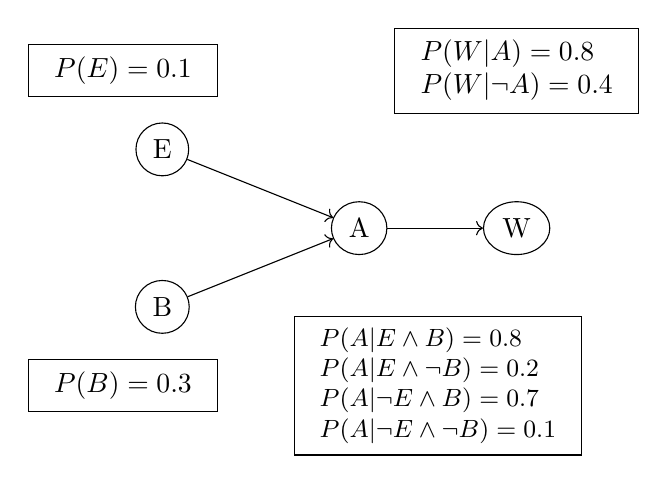
\begin{tikzpicture}
    \tikzstyle{every node}=[draw];
    \node (tab1) at (-3, -1) {
    \begin{tabular}{l}
    $P(B) =0.3$
    \end{tabular}
    };
    \node (tab2) at (-3, 3) {
    \begin{tabular}{l}
    $P(E) = 0.1$
    \end{tabular}
    };
    {\small
    \node (tab4) at (1, -1) {
    \begin{tabular}{l}
    $P(A| E \land B) =0.8$\\
    $P(A| E \land \neg B) = 0.2$\\
    $P(A|\neg E \land B) = 0.7$\\
    $P(A|\neg E \land \neg B) = 0.1$ 
    \end{tabular}
    };
    }
    \node (tab2) at (2, 3) {
    \begin{tabular}{l}
    $P(W| A) =0.8$\\
    $P(W| \neg A) = 0.4$
    \end{tabular}
    };
    \node[ellipse] (a) at (-2.5, 2) {E};
    \node[ellipse] (b) at (-2.5, 0) {B};
    \node[ellipse] (c) at (0, 1) {A};
    \node[ellipse] (d) at (2, 1) {W};
    \path[draw] [->] (a) -- (c);
    \path[draw] [->] (b) -- (c);
    \path[draw] [->] (c) -- (d);
\end{tikzpicture}
\end{center}

Suppose we would like to calculate the probability of a burglary occurring given that the alarm did not go off (i.e., $P(B|\lnot A)$.

\begin{verbatim}
Define factors f(E) f(B) f(B E A) f(A W)
E	Value
0	0.9000
1	0.1000

B	Value
0	0.7000
1	0.3000

B	E	A	Value
0	0	0	0.9000
0	0	1	0.1000
0	1	0	0.8000
0	1	1	0.2000
1	0	0	0.3000
1	0	1	0.7000
1	1	0	0.2000
1	1	1	0.8000

A	W	Value
0	0	0.6000
0	1	0.4000
1	0	0.2000
1	1	0.8000


Restrict f(B E A) to A = 0 to produce f(B E)
B	E	Value
0	0	0.9000
0	1	0.8000
1	0	0.3000
1	1	0.2000

Restrict f(A W) to A = 0 to produce f(W)
W	Value
0	0.6000
1	0.4000

Sum out W from f(W) to produce f()
Value
1.0000

Multiply f(E) f(B E) to produce f(B E)
B	E	Value
0	0	0.8100
0	1	0.0800
1	0	0.2700
1	1	0.0200

Sum out E from f(B E) to produce f(B)
B	Value
0	0.8900
1	0.2900

Multiply f(B) f() f(B) to produce f(B)
B	Value
0	0.6230
1	0.0870

Normalize: f(B)
B	Value
0	0.8775
1	0.1225
\end{verbatim}

From the last factor, we see that $P(B|\lnot A)=0.1225$.

\end{appendices}

\end{document}